% !TEX root = ../thesis.tex

\section{Results}
\label{sec:results}

% Results overview
The results of the search for a new heavy boson resonance are considered in terms of exclusion limits for the benchmark signal models described in this analysis.
These limits are model-independent, and cover spin-0, spin-1, and spin-2 resonances decaying to \WW, \WZ, and \WH.

\subsection{Exclusion Limits}

% Exclusion limits
We derive 95\% confidence-level (CL) upper limits on the resonance production cross section times branching ratio to \WW, \WZ, or \WH as a function of the mass hypothesis \MX for a narrow resonance, and compare them to expected cross sections from the benchmark models where available.
The resulting limits are shown in figures~\ref{fig:exclusion_limits_spin0}, \ref{fig:exclusion_limits_spin1}, and \ref{fig:exclusion_limits_spin2} for the spin-0, spin-1, and spin-2 signal models, respectively.
These limits are obtained for the combination of all 24 search categories, showing the observed and median expected limits with the 68\% and 95\% expected bands.

\begin{figure}[htbp]
  \centering
  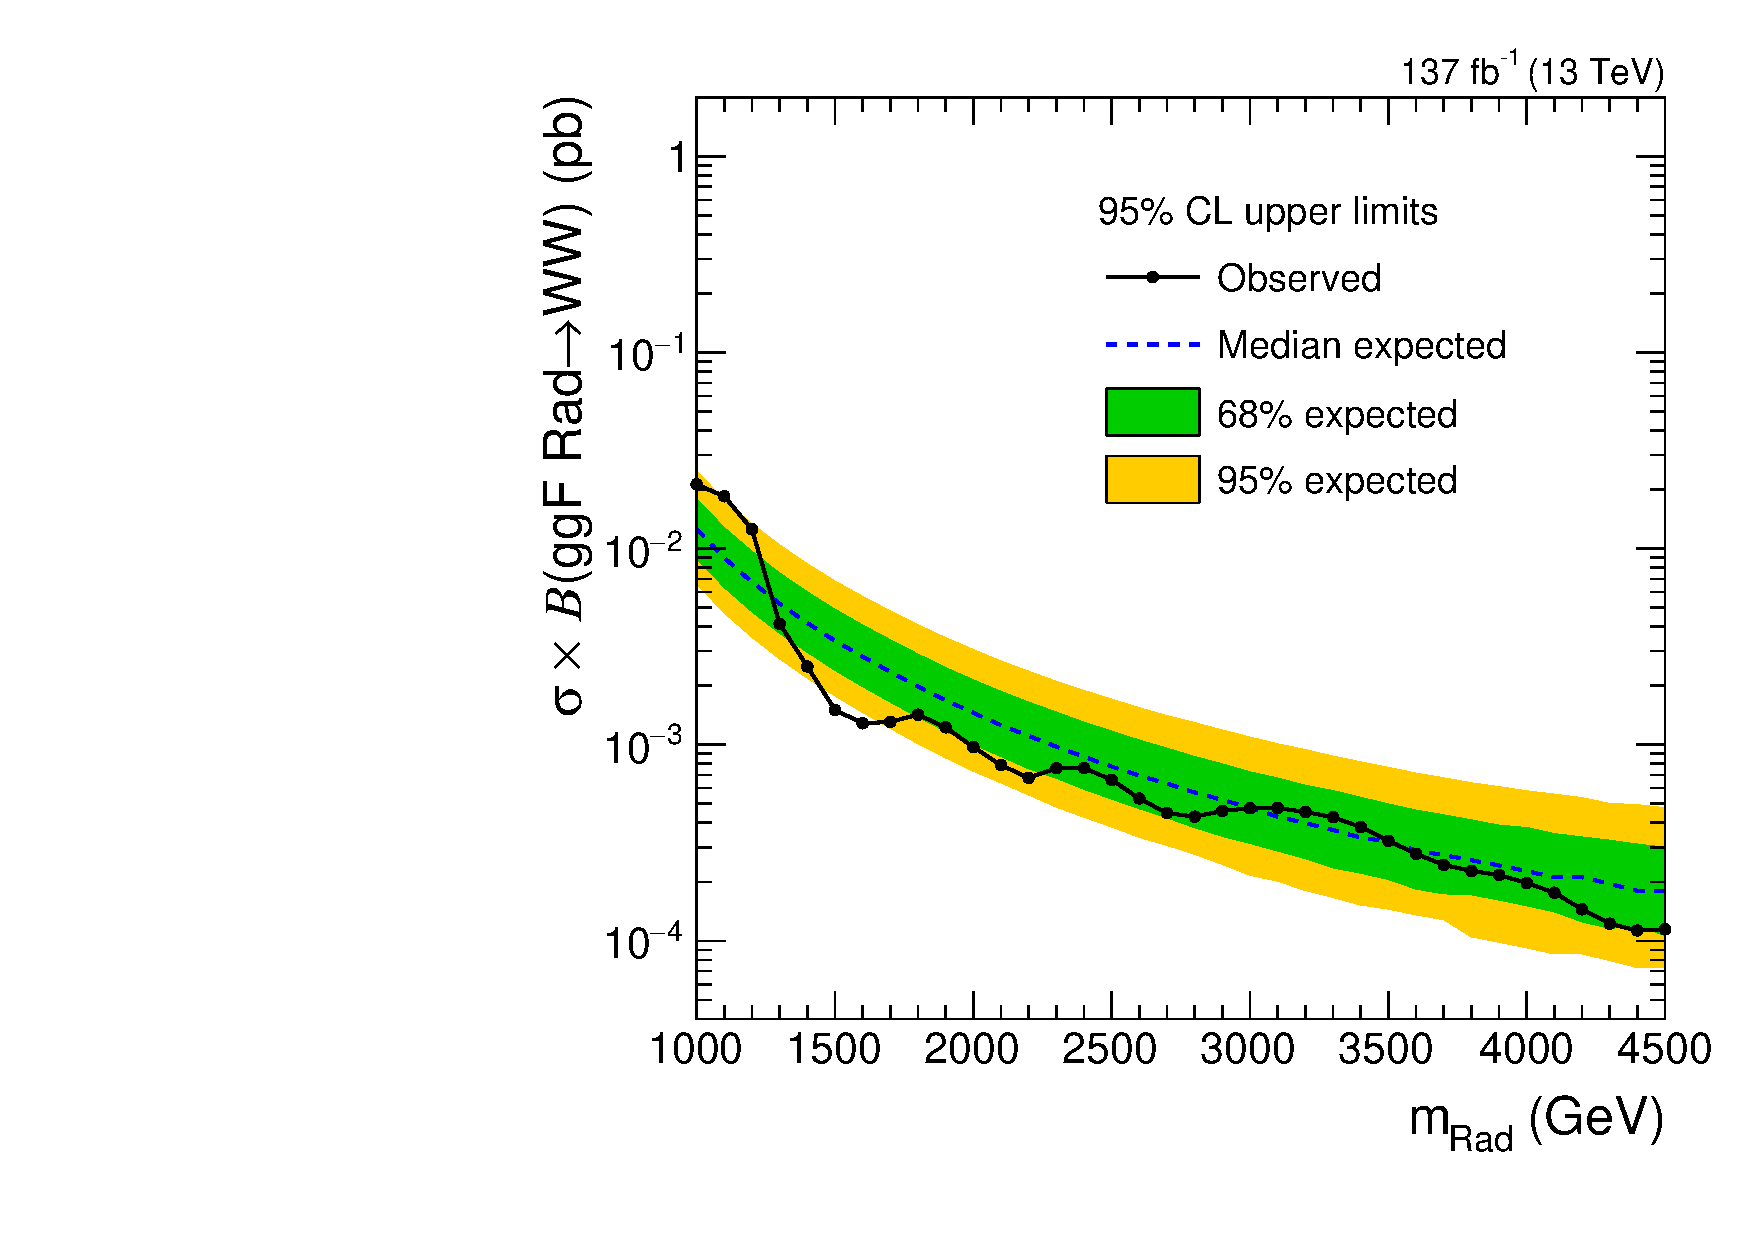
\includegraphics[width=0.3\textwidth]{fig/results/limits_RadToWW_o_74.pdf}
  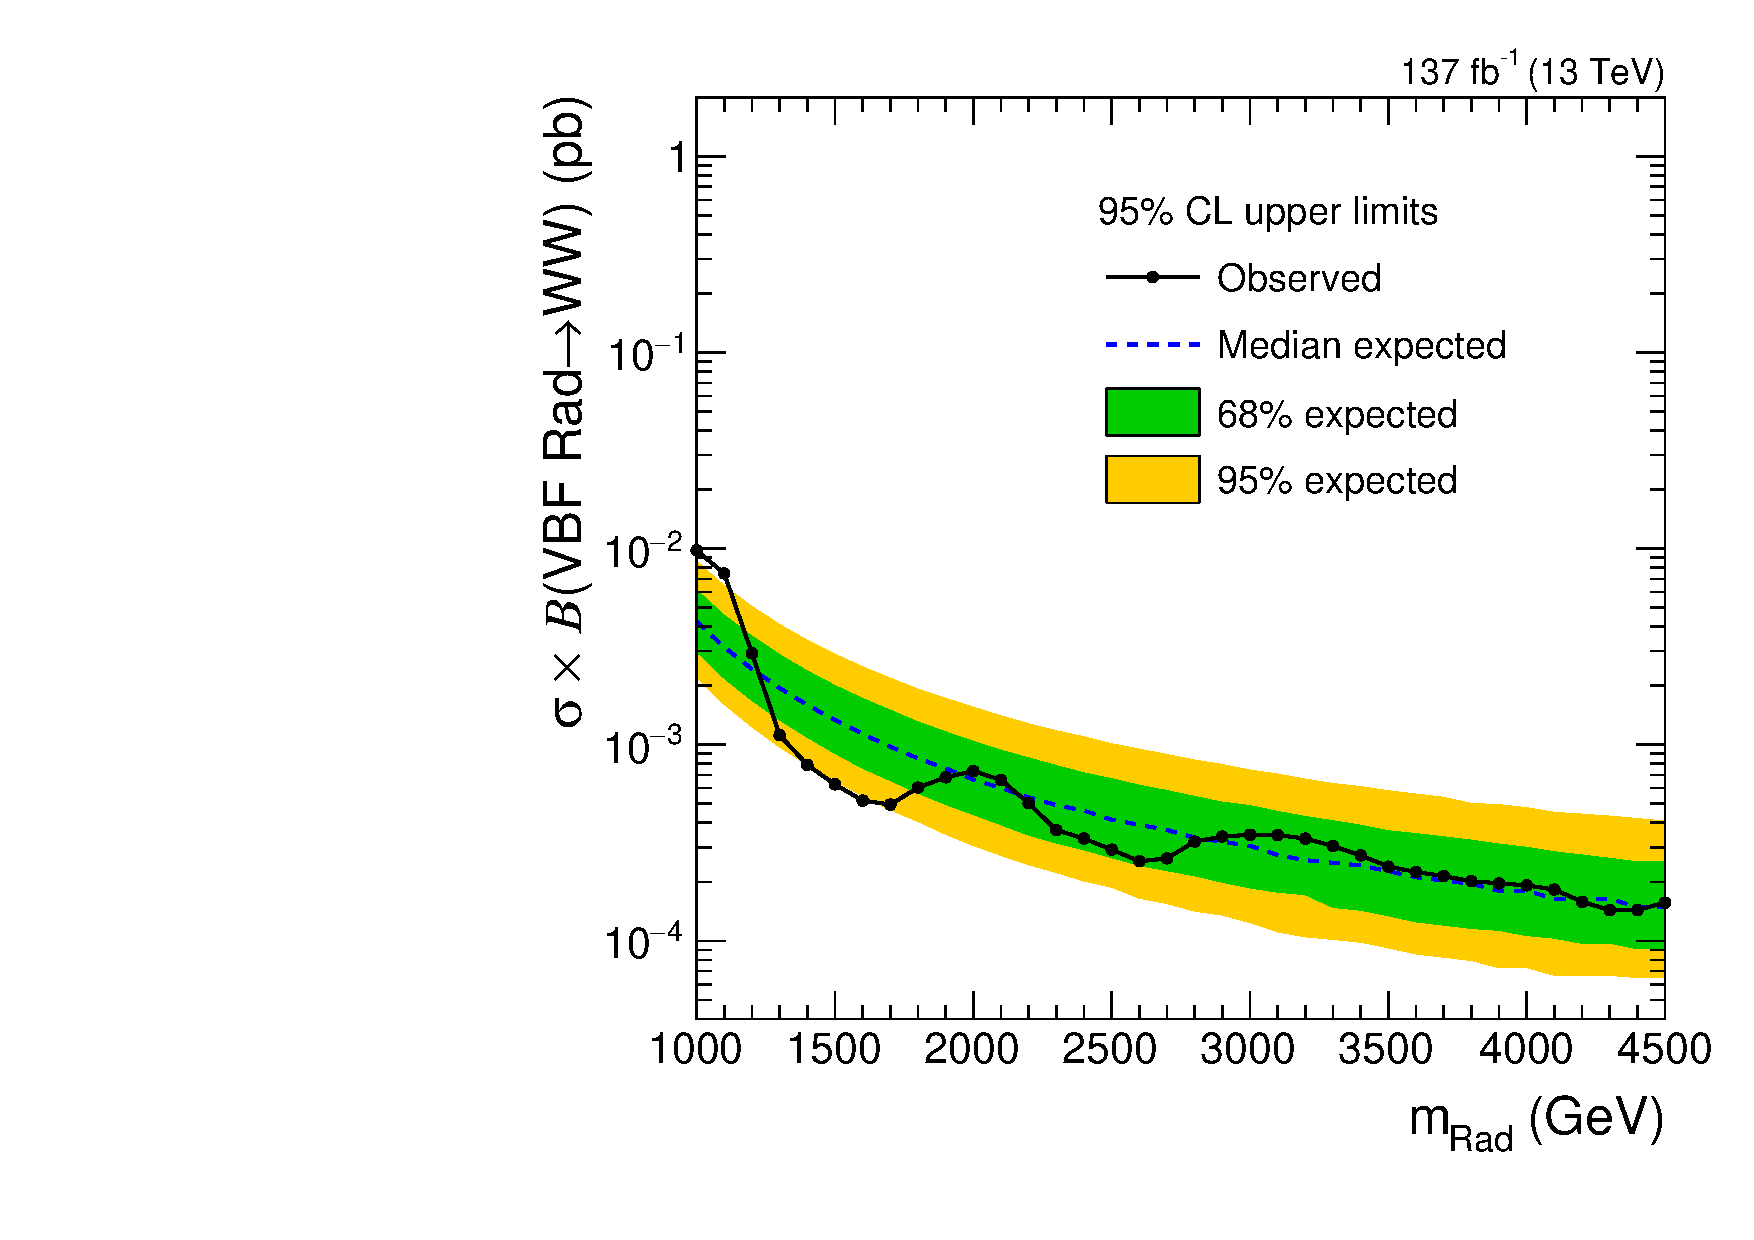
\includegraphics[width=0.3\textwidth]{fig/results/limits_VBFRadToWW_o_74.pdf}
  \caption{
    Exclusion limits on the product of the production cross section with the branching ratio for a new neutral spin-0 resonance produced via gluon-gluon fusion (left) or vector boson fusion (right) and decaying to \WW, as a function of the resonance mass hypothesis \MX.
  }
  \label{fig:exclusion_limits_spin0}
\end{figure}

\begin{figure}[htbp]
  \centering
  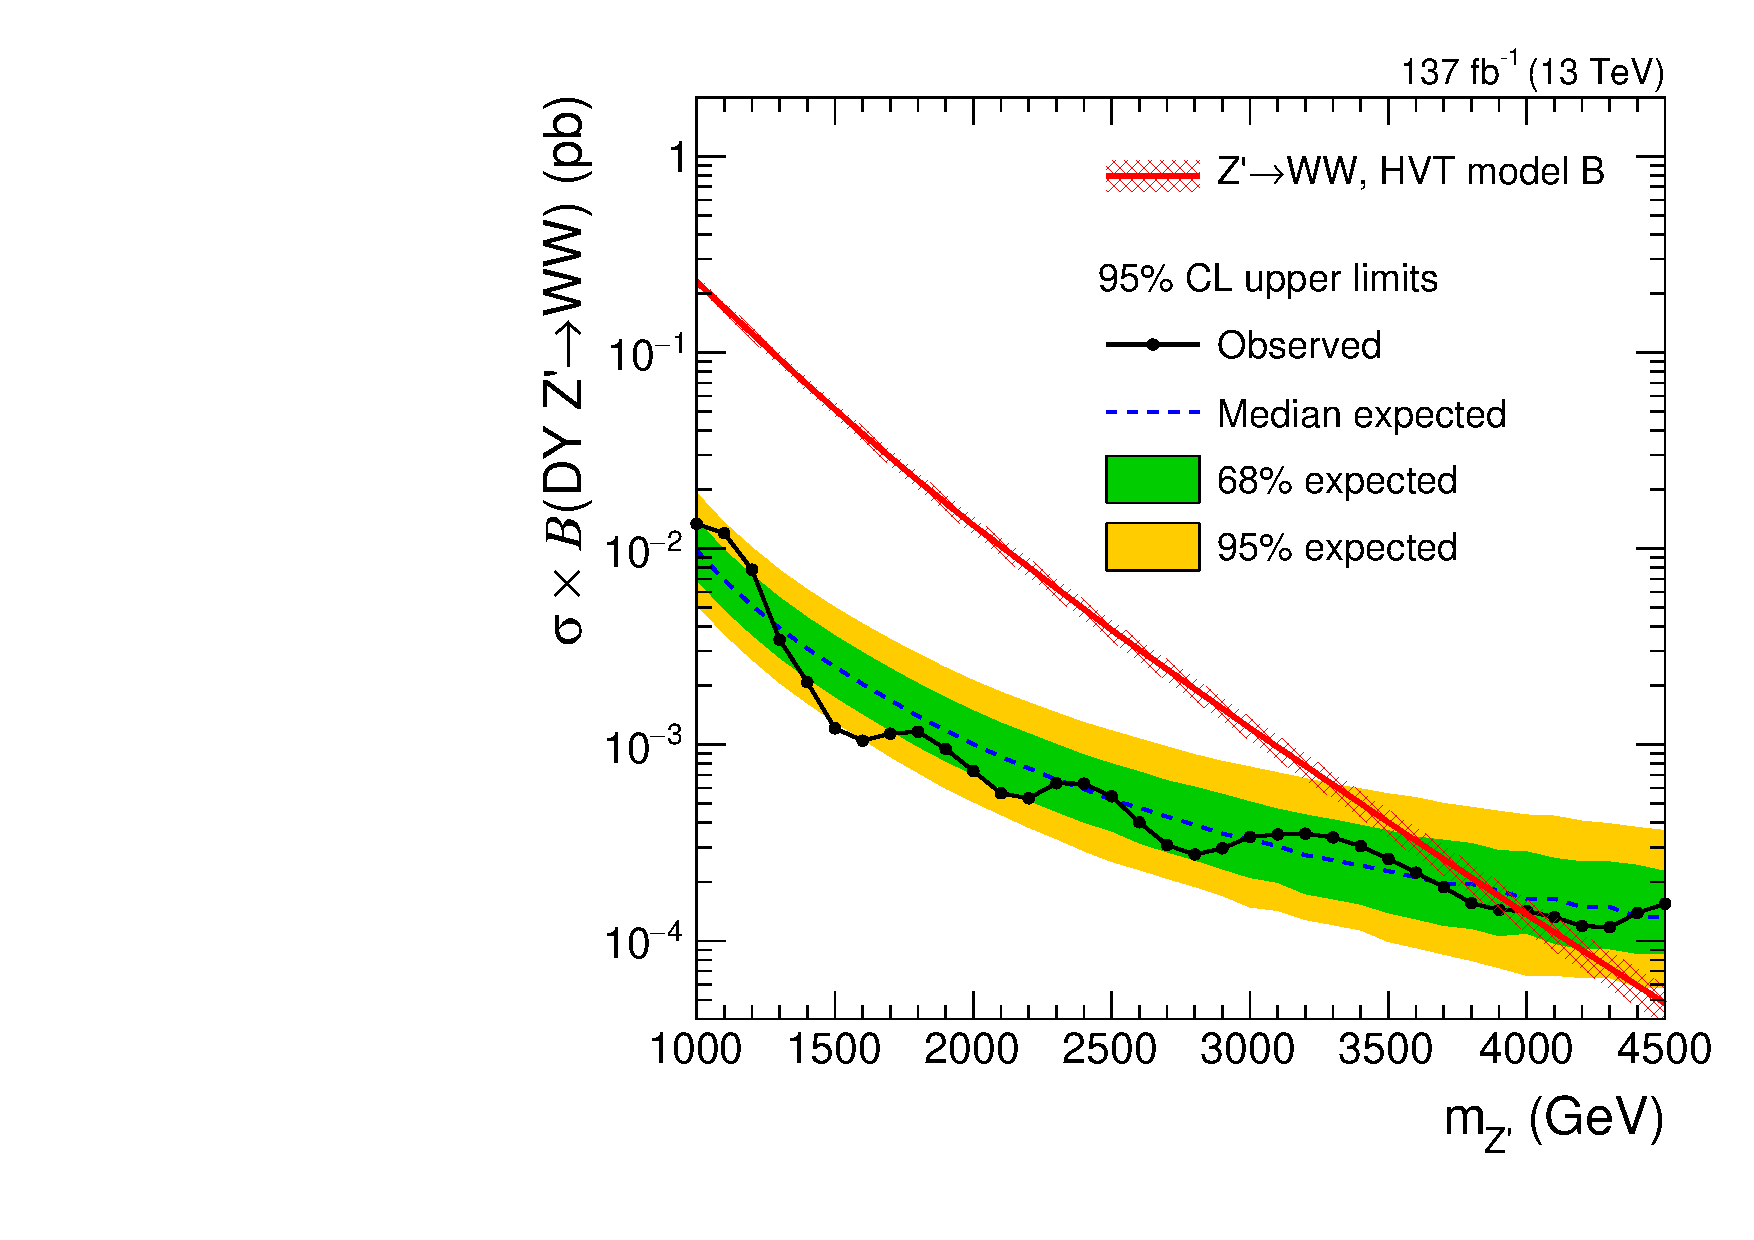
\includegraphics[width=0.3\textwidth]{fig/results/limits_ZprToWW_o_74.pdf}
  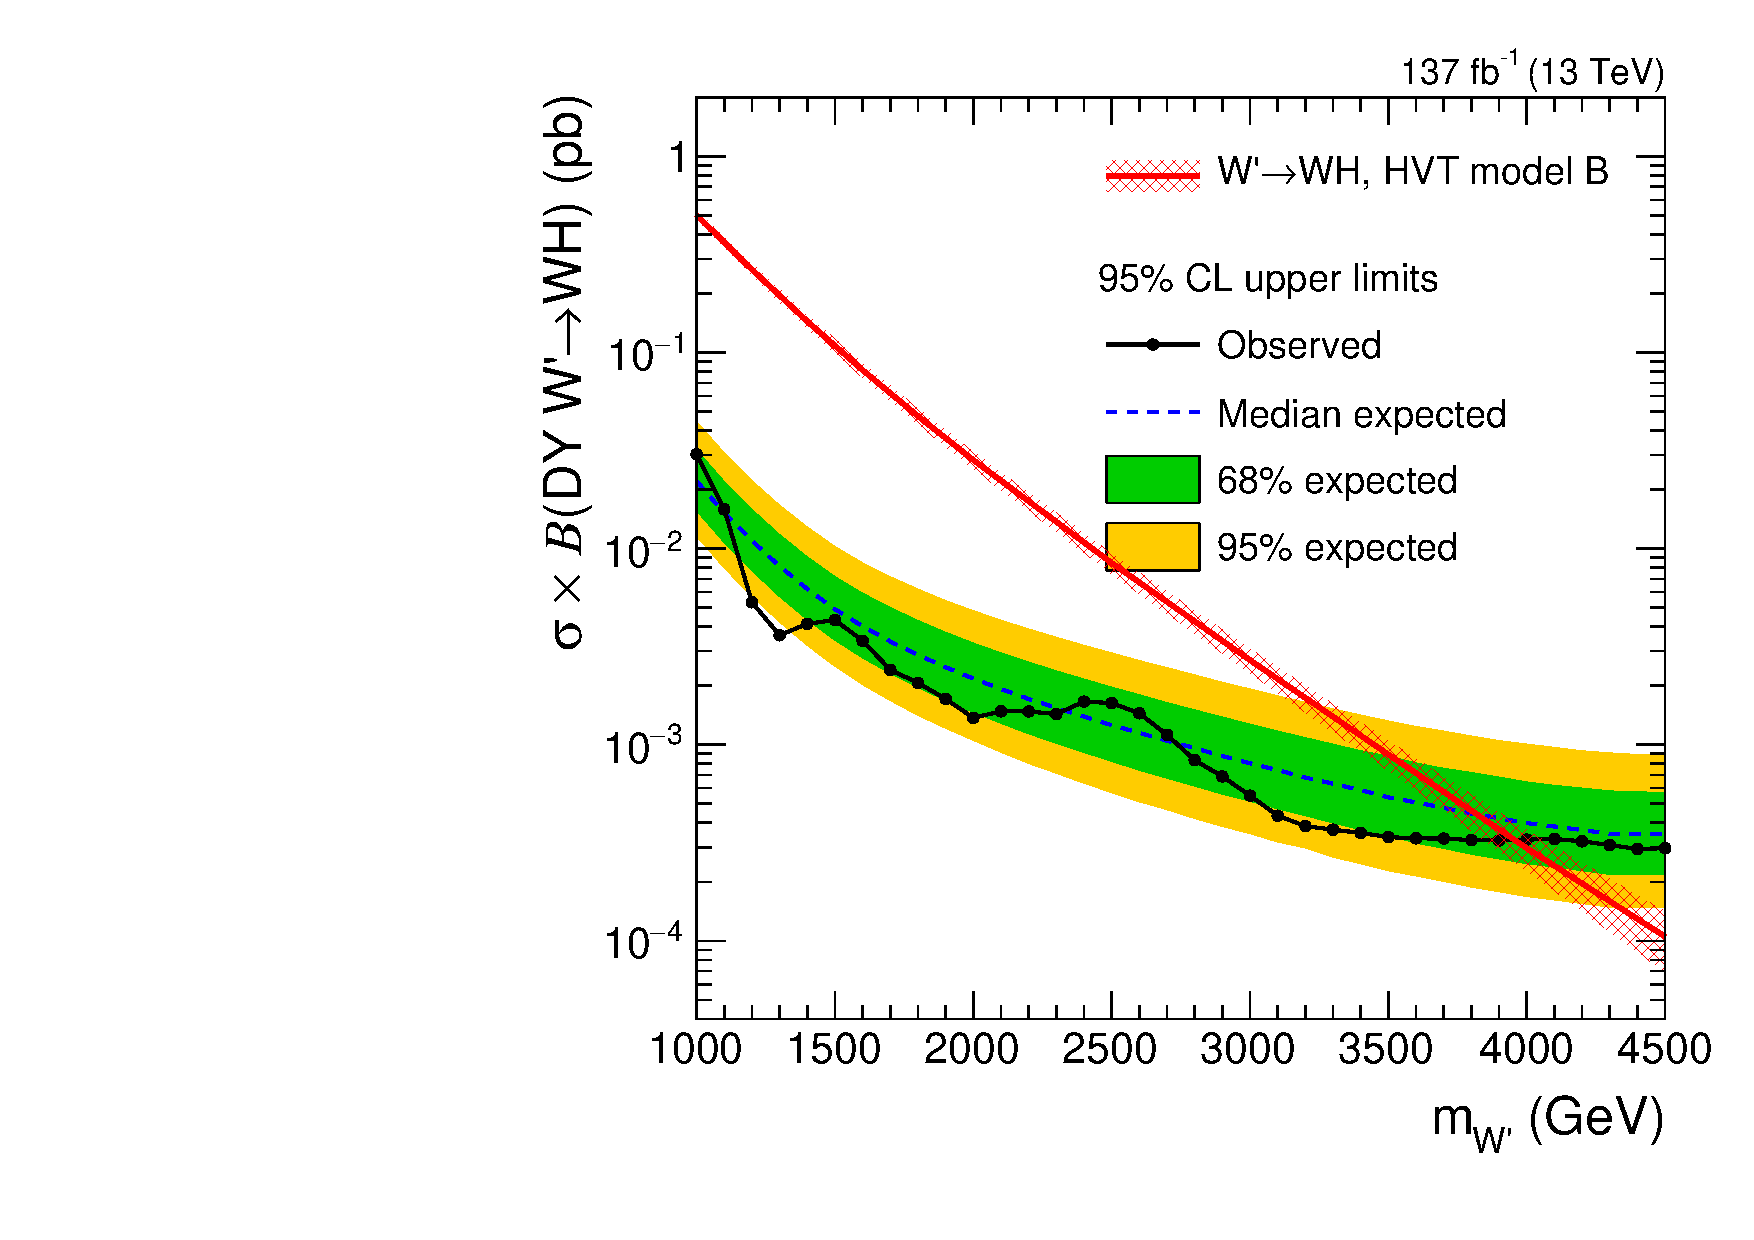
\includegraphics[width=0.3\textwidth]{fig/results/limits_WprToWH_o_74.pdf}
  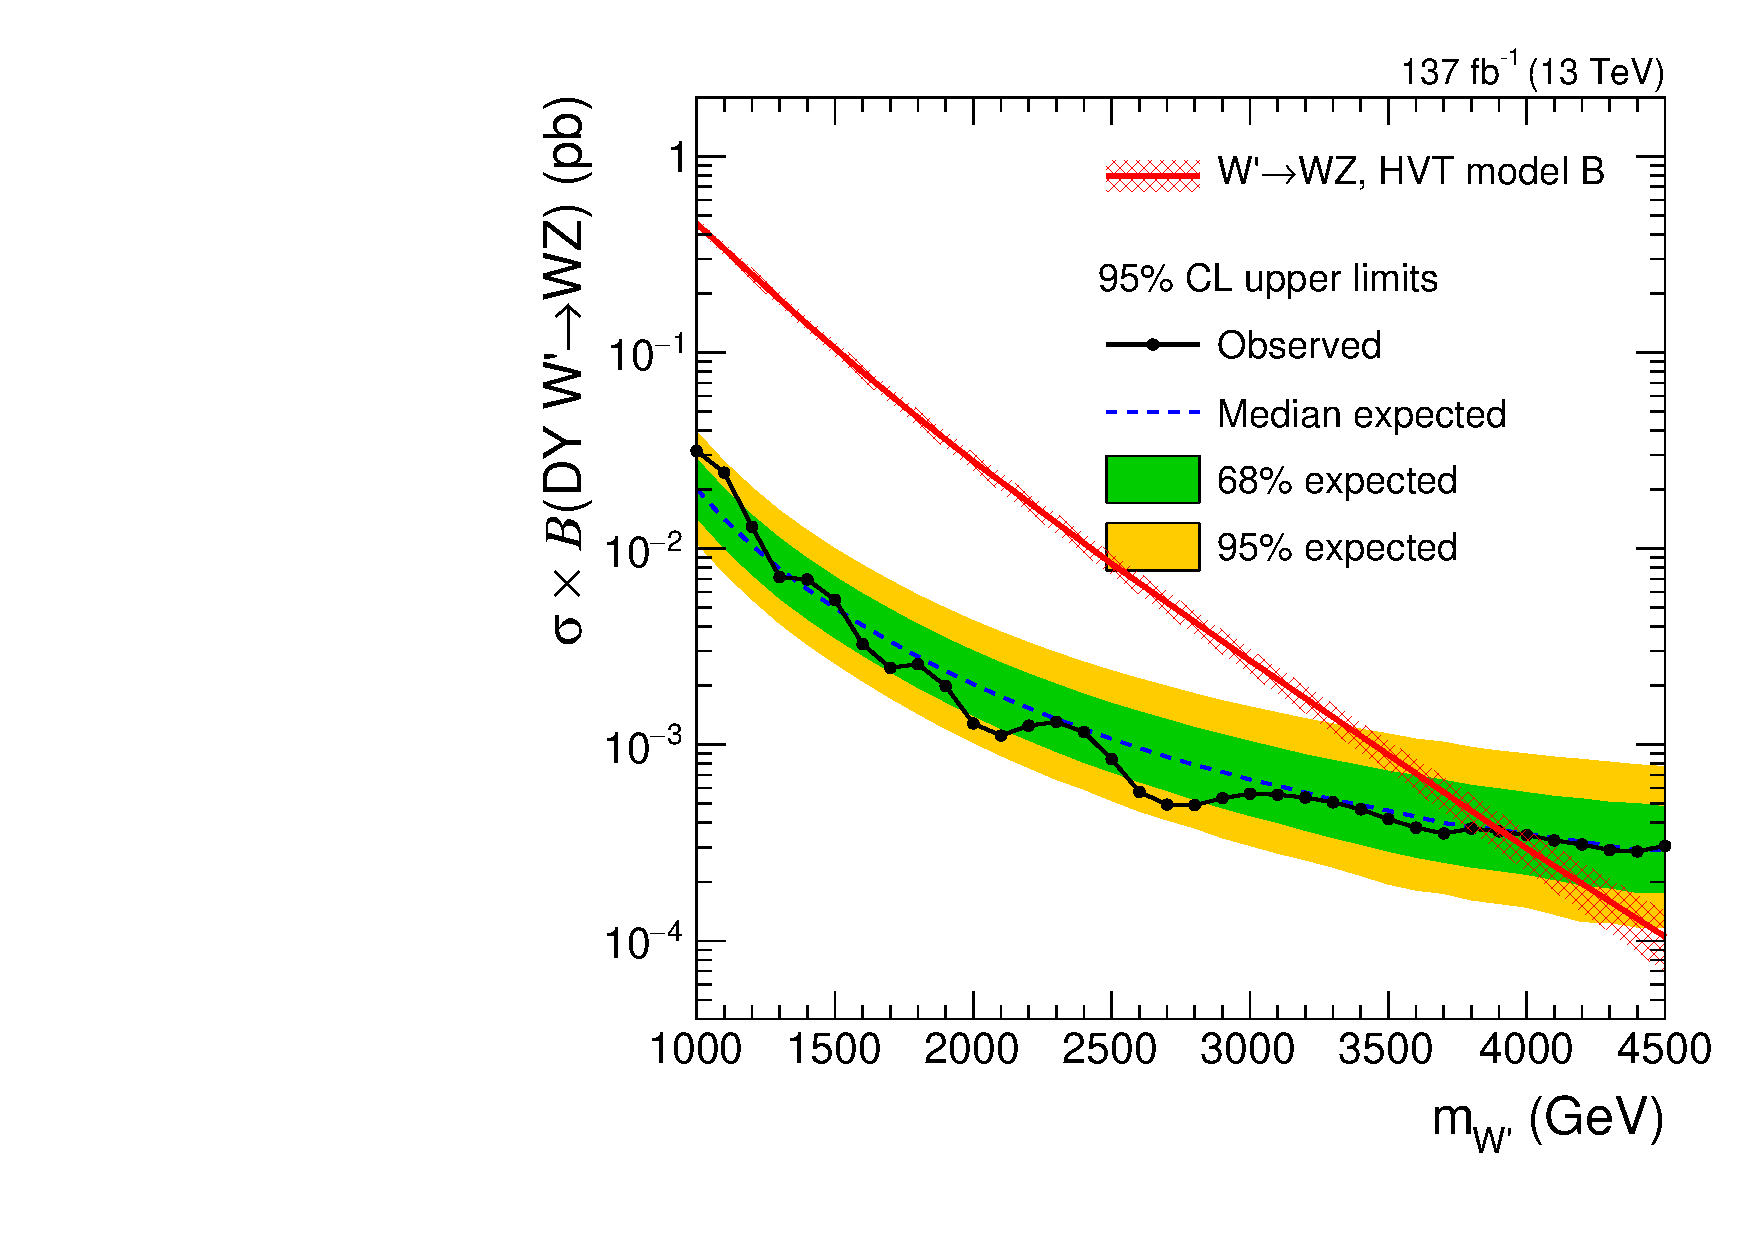
\includegraphics[width=0.3\textwidth]{fig/results/limits_WprToWZ_o_74.pdf}\\
  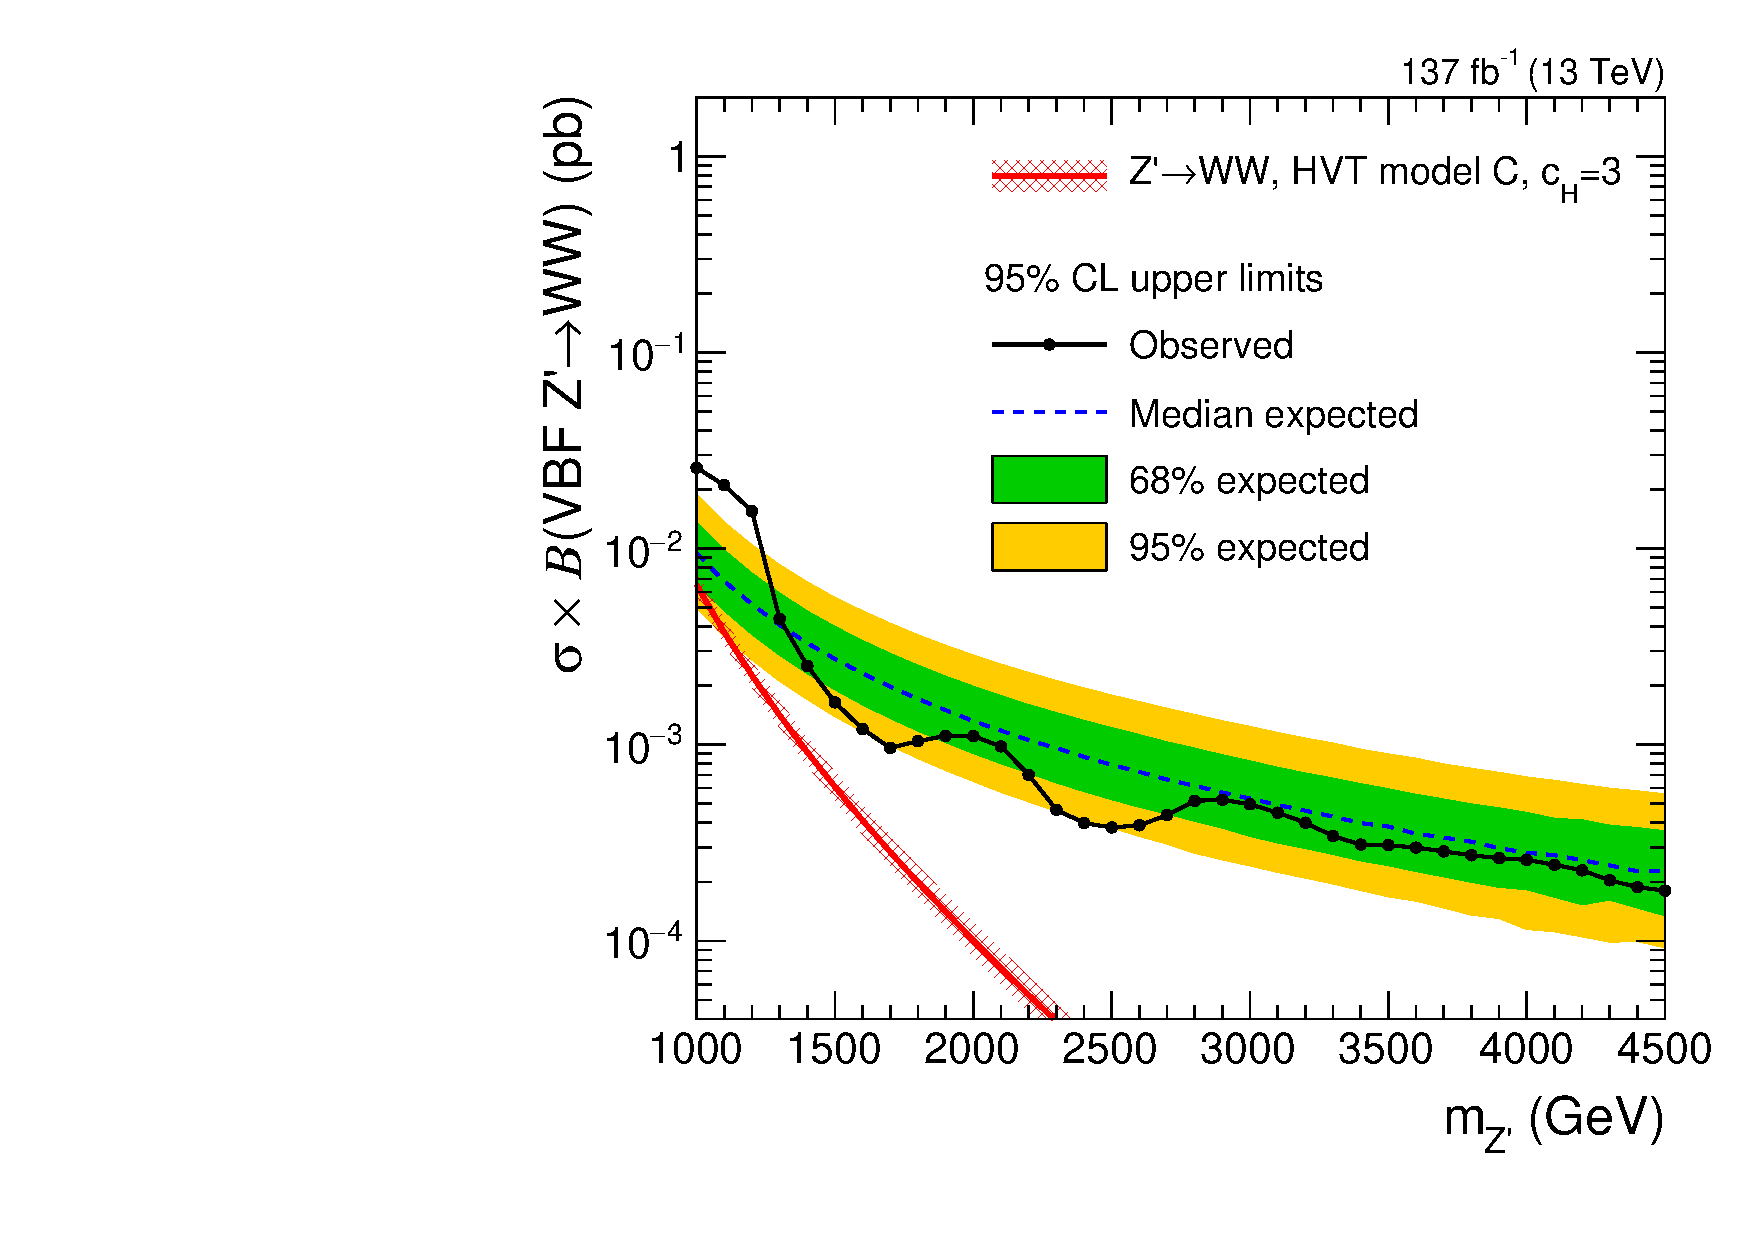
\includegraphics[width=0.3\textwidth]{fig/results/limits_VBFZprToWW_o_74.pdf}
  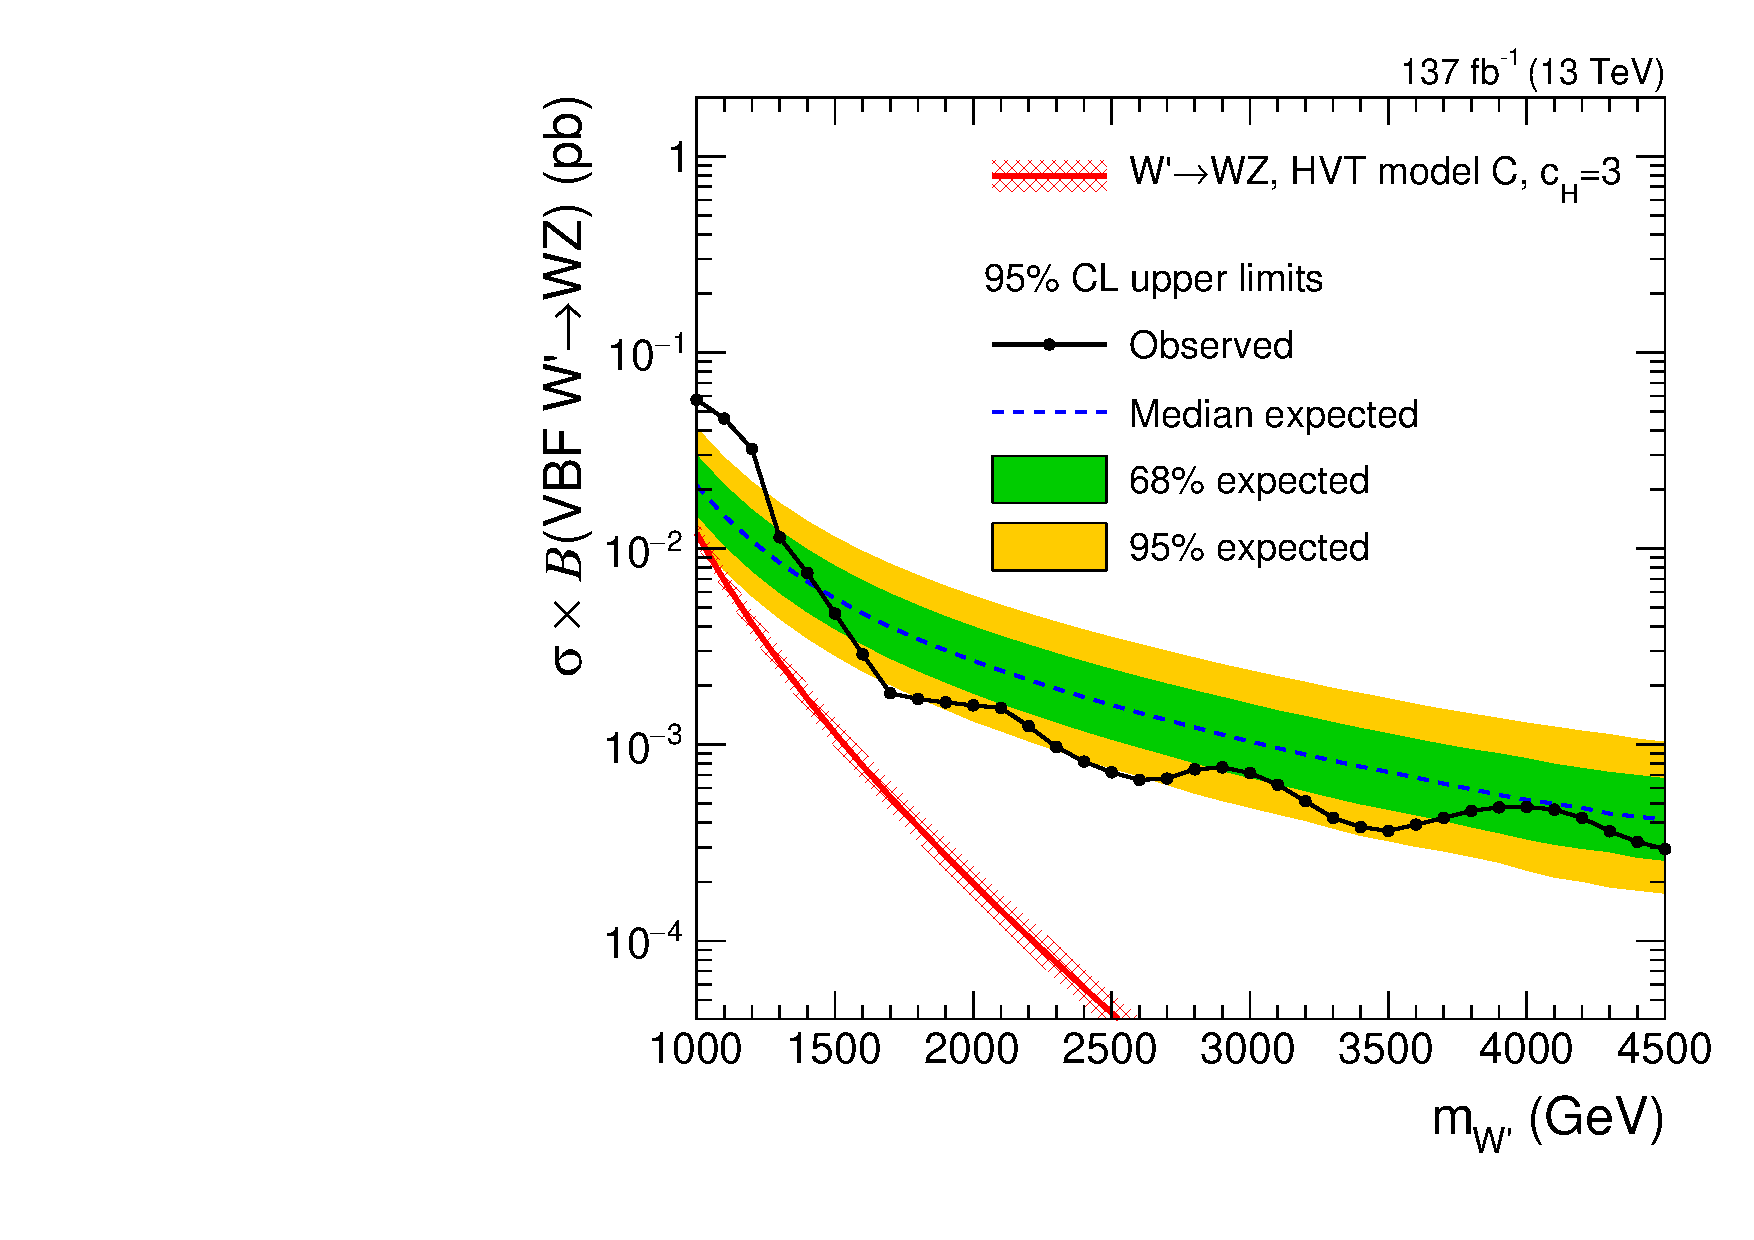
\includegraphics[width=0.3\textwidth]{fig/results/limits_VBFWprToWZ_o_74.pdf}
  \caption{
    Exclusion limits on the product of the production cross section with the branching ratio for a new neutral spin-1 resonance produced via Drell-Yan (top left) or vector boson fusion (bottom left) and decaying to \WW, for a new charged spin-1 resonance produced via Drell-Yan (top center) and decaying to \WH, and for a new charged spin-1 resonance produced via Drell-Yan (top right) or vector boson fusion (bottom right) and decaying to \WZ, as a function of the resonance mass hypothesis \MX, compared with the predicted cross sections for a \Wpr or \Zpr from HVT model B (for \DY)  or HVT model C with $c_\mathrm{H}=3$ (for \VBF).
    The signal cross section uncertainties are shown as red cross-hatched bands.
  }
  \label{fig:exclusion_limits_spin1}
\end{figure}

\begin{figure}[htbp]
  \centering
  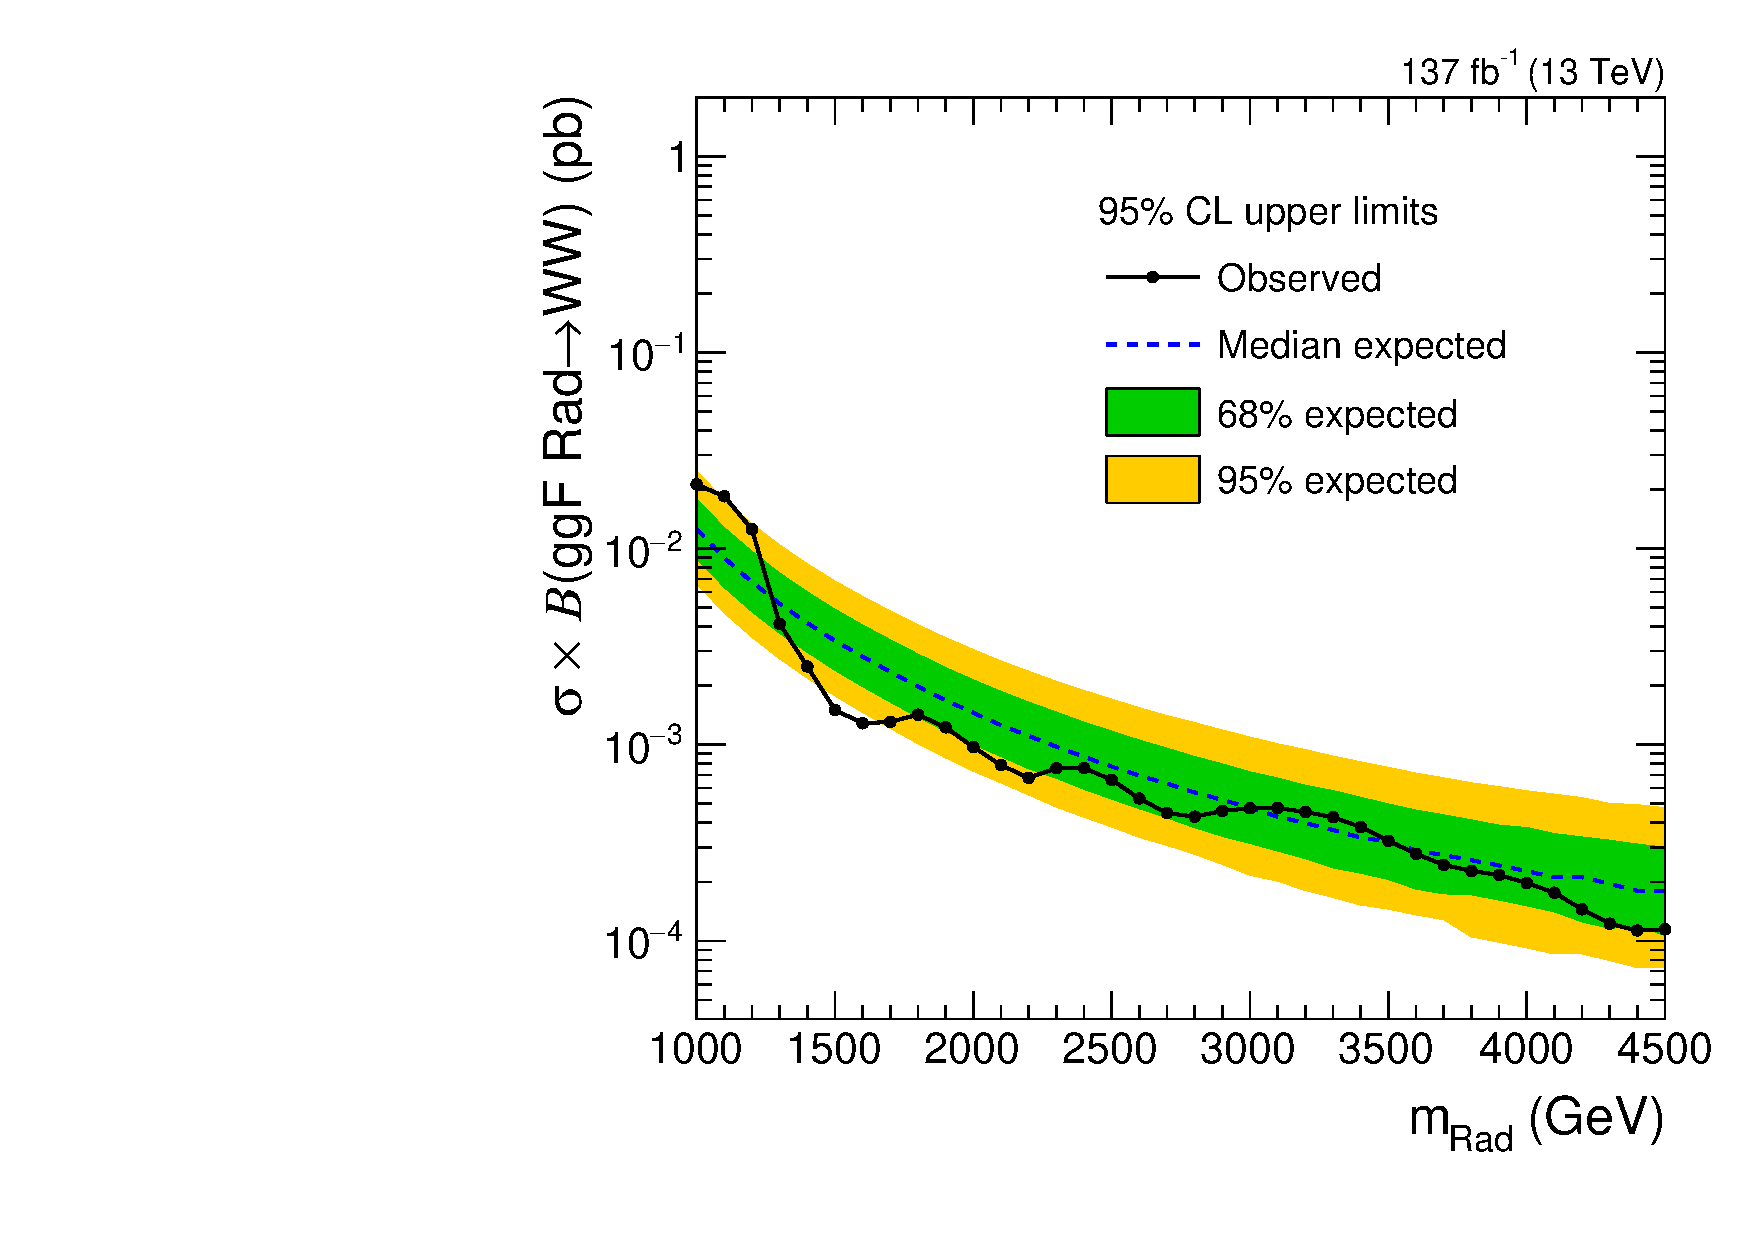
\includegraphics[width=0.3\textwidth]{fig/results/limits_RadToWW_o_74.pdf}
  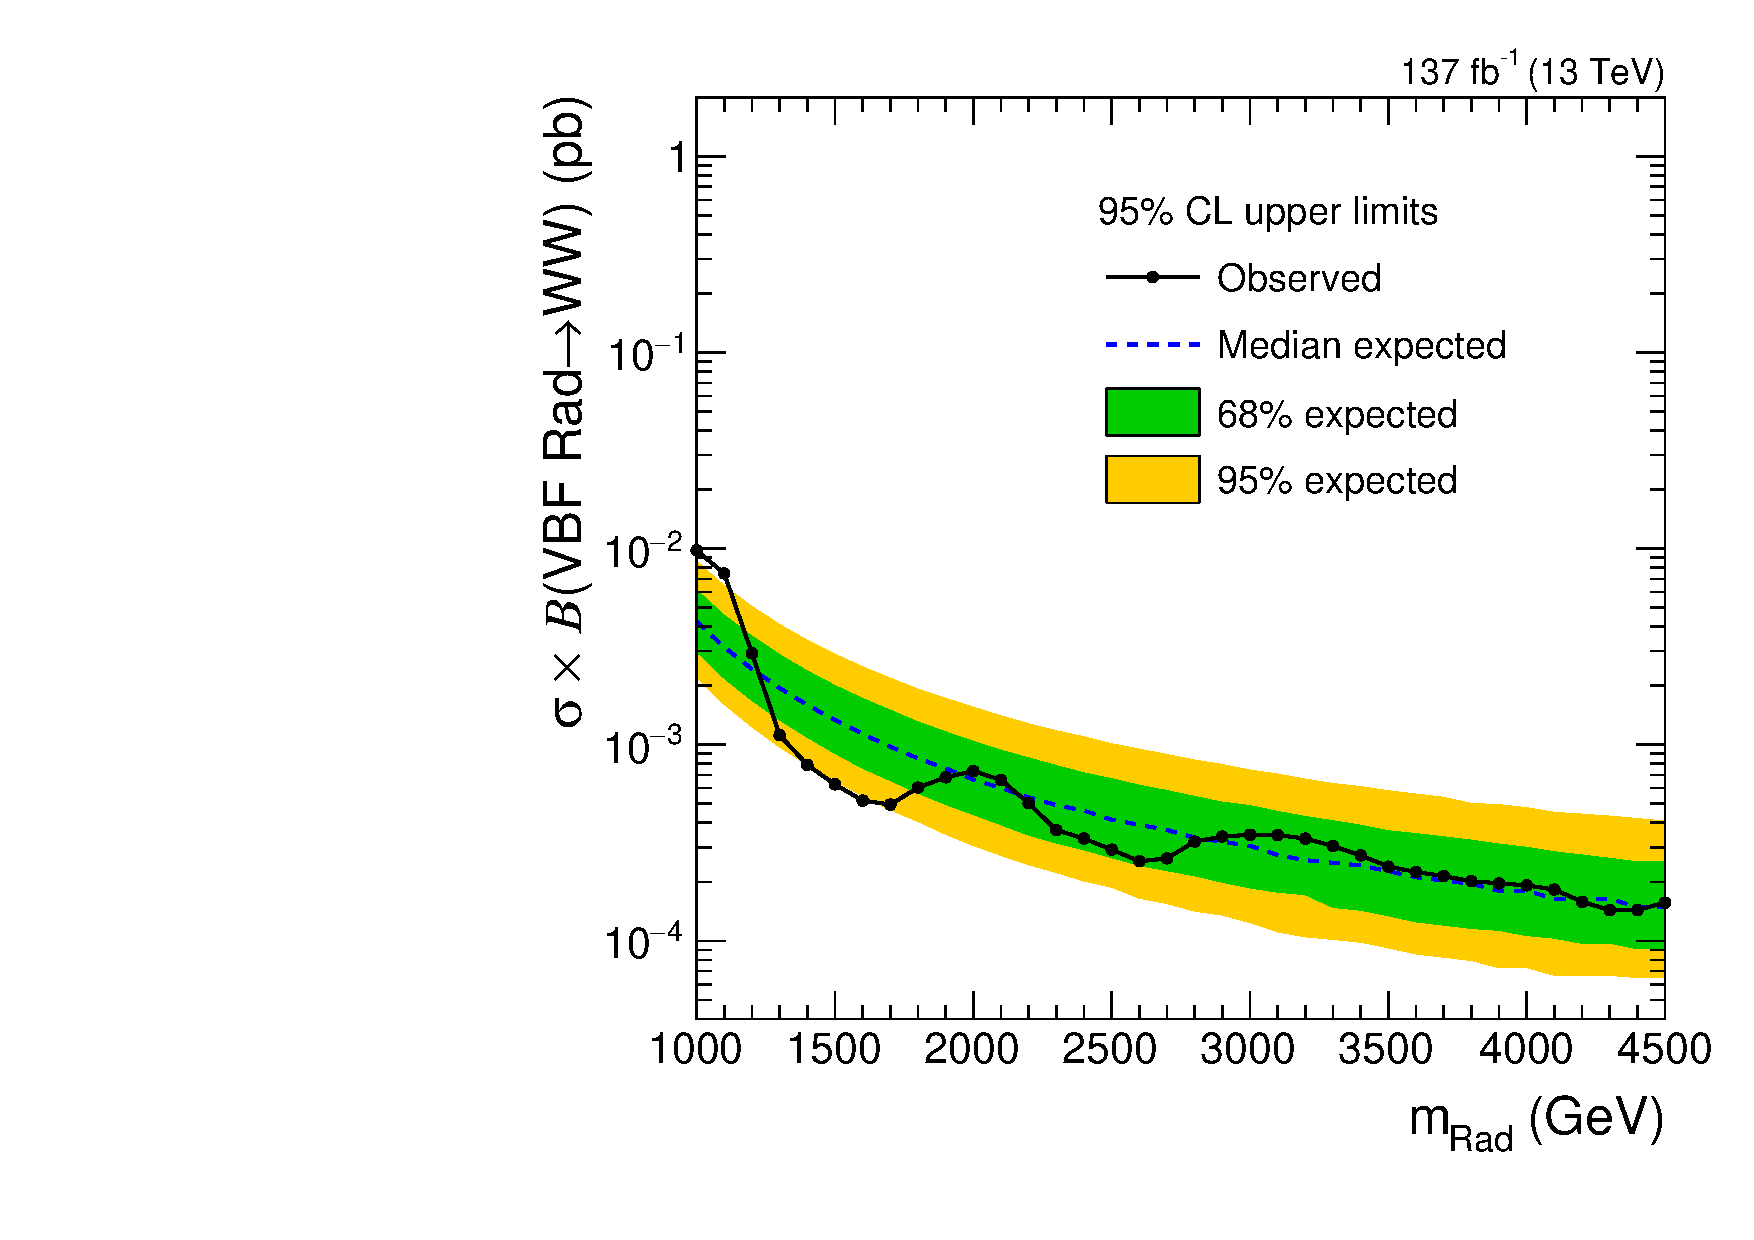
\includegraphics[width=0.3\textwidth]{fig/results/limits_VBFRadToWW_o_74.pdf}
  \caption{
    Exclusion limits on the product of the production cross section with the branching ratio for a new neutral spin-2 resonance produced via gluon-gluon fusion (left) or vector boson fusion (right) and decaying to \WW, as a function of the resonance mass hypothesis \MX, compared with the predicted cross sections for a spin-2 bulk graviton with curvature $\tilde{k}=0.5$.
    The signal cross section uncertainties are shown as red cross-hatched bands.
  }
  \label{fig:exclusion_limits_spin2}
\end{figure}
